%!TEX root=../../root.tex

\section{Lezione 15}
\subsection{Problema dell'appartenenza per TM}
Chiameremo il problema dell'appartenenza per macchine di Turing $A_{TM}$. Questo è anche primo esempio di macchina universale, in pratica un calcolatore. Questa macchina prende in input un' altra macchina e un suo input e il risultato della computazione dipende dal risultato dell'esecuzione della macchina presa in input sul suo input.
\[
	A_{TM} = \{ <T, x> | x \in L(T)\}
\]
$A_{TM}$ è Turing-Riconoscibile ma non decidibile.
[immagine dei Problemi di decisione che includono i Turing-riconoscibili, che includono i decidibili]
\subsection{Teorema}
\[
	A_{TM}\ non\ decidibile
\]
\textit{Dimostrazione:} Supponiamo per assurdo che $A_{TM}$ sia decidibile $\Rightarrow \exists T \in TM \quad t.c. \quad L(T)=A_{TM}$ e si ferma sempre \\
\begin{equation*}
	T(<M,w>) =
	\begin{cases}
   	accetta \ se \ M \ accetta \ w\\rifiuta \ altrimenti
   	\end{cases}
\end{equation*}
Considero la macchina T' uguale a T ma con le uscite invertite:
\begin{equation*}
	T'(<M,w>) =
	\begin{cases}
   	accetta \ se \ w \notin L(M)\\rifiuta \ se \ w \in L(M)
   	\end{cases}
\end{equation*}
Considero T'' che si comporta come T' ma prende in input due codifiche di macchine

\begin{equation*}
	T''(<M,<M'>>) =
	\begin{cases}
   	accetta \ se \ <M'> \notin L(M)\\rifiuta \ se \ <M'> \in L(M)
   	\end{cases}
\end{equation*}

\begin{tabular}[left]{ c | c c c c }
	T'' & $<M1>$ & $<M2>$ & $<M3>$ & $\cdots$ \\
	\hline
	M1 & acc & rif & acc & $\cdots$ \\
	M2 & rif & rif & acc & $\cdots$ \\
	M3 & acc & acc & rif & $\cdots$ \\
	$\vdots$ & $\vdots$ & $\vdots$ & $\vdots$ & $\vdots$ 
\end{tabular} \\ \\
Descriviamo ora la diagonale della macchina T'' con una macchina T'''
\begin{equation*}
	T'''(<M>) =
	\begin{cases}
   	accetta \ se \ <M> \notin L(M)\\rifiuta \ se \ <M> \in L(M)
   	\end{cases}
\end{equation*}
Tra le macchine M, posso considerare anche T''', per cui T''' diventa:
\begin{equation*}
	T'''(<T'''>) =
	\begin{cases}
   	accetta \ se \ <T'''> \notin L(T''')\\rifiuta \ se \ <T'''> \in L(T''')
   	\end{cases}
\end{equation*}
Qui arriviamo a una contraddizione, poiché T''' ci dice che:
\begin{center}
	$<T'''> \in L(T''') \Leftrightarrow <T'''> \notin L(T''')$ \footnote{Paradosso di Russel: Siano F = $\{X \mid X \text{ è infinito}\}$, E = $\{X \mid X \text{ è finito}\}$ e R = $\{X \mid X \notin X\}$. \\
	$F \in R? \text{ Si, poiché F è a sua volta un insieme infinito}$ \\
	$E \in R? \text{ No, perché E è un insieme infinito}$ \\
	$R \in R? \ R \in R \Rightarrow R \notin R, ma R \notin R \Rightarrow R \in R $ }
\end{center} 
\subsection{Teorema}
Se L è Turing-Riconoscibile e anche $\overline{L}$ lo è, allora L è decidibile \\
\textit{Dimostrazione:}
\[
	\exists T,T' \in TM \mid L(T)=L \ e \ L(T') = \overline{L}
\] 
\begin{figure}[H]
	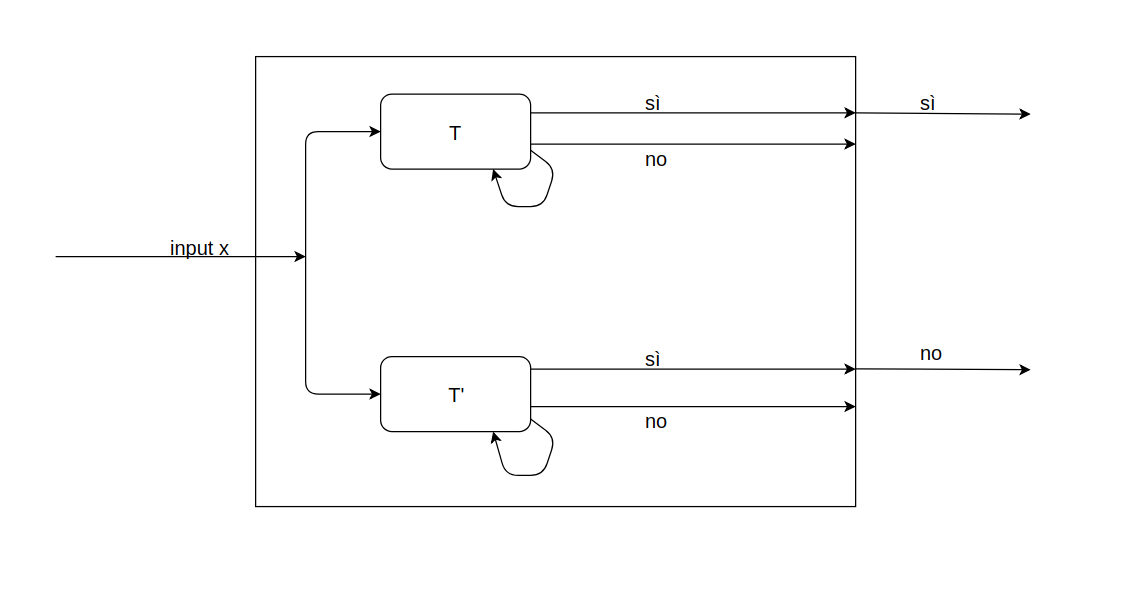
\includegraphics[scale=0.35]{automa-parallelo}
\end{figure}
Descrizione di M:
\begin{description}
	\item \textit{input}: x
	\item \textit{output}: s\`i se x $\in$ L, no altrimenti 
	\item \textit{Descrizione ad alto livello}:
		\begin{enumerate}
			\item fai una mossa di T sul primo nastro, se T accetta, allora accetta
			\item fai una mossa di T' sul secondo nastro, se T' accetta, allora rifiuta
		\end{enumerate}			
\end{description}

\subsubsection{Corollario}
\[
	\overline{A_{TM}}\ non\ \text{è}\ Turing-Riconoscibile
\]
\textit{Dimostrazione:} 
$A_{TM}$ è Turing-Riconoscibile e quindi se $\overline{A_{TM}}$ fosse Turing-Riconoscibile dovrei dedurre che $A_{TM}$ sia decidibile. \\
\\
$A_{TM} = \{ <M,w> \ \mid \ w \in L(M) \ e \ M \in TM \}$ \\
\\
$\overline{A_{TM}} = \{ X \mid \text{X non codifica M,w} \} \cup \{ <M,w> \mid M \in TM \text{ e } w \notin L(M) \}$
\subsection{Il problema della fermata}
$Halt_{TM} = \{ <M,w> \ e \ M \in \text{TM e M si ferma su w} \}$ \\
\textit{$Halt_{TM}$ non è decidibile} \\
\textit{Dimostrazione: } Per assurdo supponiamo che $Halt_{TM}$ sia decidibile
\begin{equation*}
	\exists T \in TM \text{ tale che } T(<M,w>) = 
	\begin{cases} 
		\text{accetta se M si ferma su w} \\ 
		\text{rifiuta se M non si ferma}
	\end{cases} 
\end{equation*}
T': 
\begin{description}
\item \textit{input}: $<M, w>$
\item \textit{output}: sì se $w \in L(M)$, no altrimenti
\item \textit{descrizione}:
\begin{enumerate}[label*=\arabic*.]
\item esegue $T$ su $<M,w>$

\item se $T$ accetta, allora $M$ si ferma su $w$, quindi:

\begin{enumerate}[label*=\arabic*.]

\item esegue $M$ su $w$

\item se $M$ accetta $w$, allora accetta $<M,w>$

\item se $M$ rifiuta $w$, allora rifiuta

\end{enumerate}

\item se $T$ non accetta $<M,w>$ allora rifiuta

\end{enumerate}
\end{description}

Quindi per ogni codifica di macchina e input $<M, w>$ abbiamo che:

\begin{gather*}
	<M,w> \ \in \ L(T') \ se \ w \in L(M)\\
	<M,w> \ \notin \ L(T') \ se \ w \notin L(M)
\end{gather*}
Ovvero $T'$ decide $A_{TM}$, sfruttando $T$, ma abbiamo dimostrato che $A_{TM}$ non è decidibile, quindi $T$ non può esistere [Contraddizione].

\subsection{Mapping Reduction}
\begin{figure}[H]
	\centering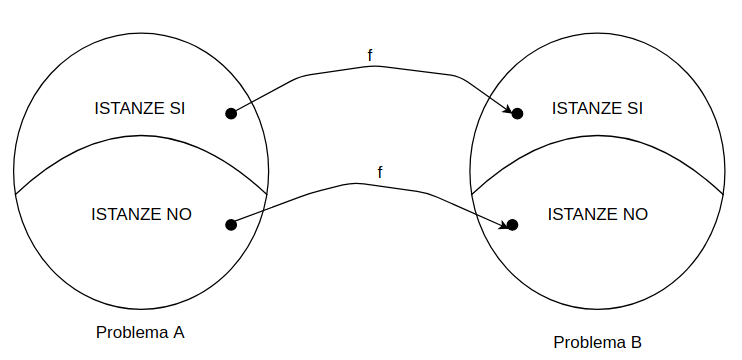
\includegraphics[scale=0.4]{riduzione}
\end{figure}
Siano $A,B \subseteq \Sigma^{\star}$ due problemi, con $A \le_{m} B$ si indica che il problema A "\textit{si riduce}" al problema B.
\begin{center}
	$A \le_{m} B \iff \exists f: \Sigma^{\star} \rightarrow \Sigma^{\star} \text{ tale che:}$
	\begin{enumerate}
		\item $f$ deve essere calcolabile ovvero $ \exists \ T_{f} \in TM \text{ t.c ricevendo } x \in \Sigma^{\star} \text{ in input scrive } $\\
$ f(x) \text{ sul nastro e si ferma}$ \\
		\item $x \in A \Leftrightarrow f(x) \in B$
	\end{enumerate}
\end{center}

\subsubsection{Teorema}

Se $A \le_{m} B$ e B è decidibile, allora $A$ è decidibile

\textit{Dimostrazione:} \\
$A \le_{m} B \Rightarrow \exists \text{f calcolabile x} \in A \Leftrightarrow f(x) \in B$
\begin{fleqn}
    \begin{align*}
		B \text{ è decidibile} \Rightarrow \exists T_{B} \in TM \ t.c. T_{B}(x) =
		\begin{cases}
			\text{accetta se x è in B} \\ \text{rifiuta altrimenti}
		\end{cases}
	\end{align*}
\end{fleqn}
Combino le due macchine:
\begin{figure}[H]
	\centering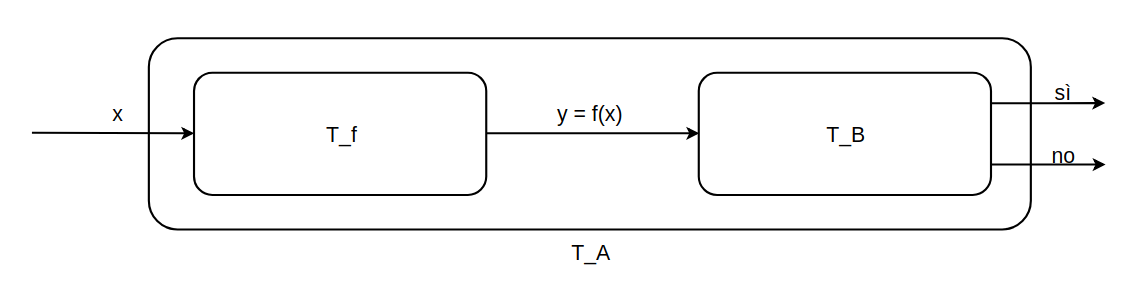
\includegraphics[scale=0.35]{automa-serie.png}
\end{figure}
\subsection{Teorema}

$A \le_{m} \text{B e supponiamo che A sia non decidibile, allora B non è decidibile}$ \\
\textit{Dimostrazione:}

Per assurdo se B fosse decidibile allora A sarebbe decidibile contro l'ipotesi \\
\\
\paragraph*{Esempio}
Sia $E_{TM}$ il linguaggio delle codifiche delle macchine che riconosco almeno una parola. Più formalmente: 
\[
	E_{TM} = \{ \ <T>  \ \mid \ T  \in TM \land L(T) \not= \emptyset \ \}
\]
Dimostriamo che $E_{TM}$ non è decidibile per riduzione utilizzando il seguente teorema: dato $A$ non decidibile se $A \le_{m} B$ allora $B$ non è decidibile.\\
Quindi se riduciamo $A_{TM}$ ad $E_{TM}$ abbiamo dimostrato che $E_{TM}$ non è decidibile poiché $A_{TM}$ non è decidibile.\\
Definiamo una macchina che calcola la funzione di riduzione di cui abbiamo bisogno. Questa macchina prende in input lo stesso input di $A_{TM}$, ossia la codifica di una macchina $M$ e di un suo input $w$ e fornisce in output la codifica di un' altra macchina $T$.
\[
	<M,w> \ \xrightarrow{f} \ <T>
\]
Sia $R_f$ la macchina che calcola la funzione di riduzione. Essa è costruita nel seguente modo:
\begin{description}
	\item \textit{Input:} $<M,w>$
	\item \textit{Output:} $<T>$
	\item \textit{Descrizione:} costruisce T come descritto di seguito.
\end{description}
T:
\begin{description}
	\item \textit{Input:} $x \in \Sigma^{\star}$
	\item \textit{Output:} s\`i se $w \in L(M) \Rightarrow L(T) = \Sigma^{\star}$, no se $w \notin L(M) \Rightarrow$ (w è rifiutata da M o M non si ferma)
	\item \textit{Descrizione:}
	\begin{enumerate}
		\item Esegui M su w
		\item Se M accetta w $\rightarrow$ accetta x
		\item Se M rifiuta w $\rightarrow$ rifiuta x
	\end{enumerate}
	\item \textit{Correttezza:}
		\item Se $w \in L(M)$ allora $L(T) = \Sigma^{\star}$, poiché $T\ \forall x \in \Sigma^{\star}$ accetta $x$ e quindi $E_{TM}$ risponderà sì.
		\item Se $w \notin L(M)$ allora $
			\begin{cases}
				\text{w è rifiutata da M} \\ \text{M non si ferma su w}
			\end{cases}
			\rightarrow L(T) = \emptyset \text{ e quindi } E_{TM} \text{ risponderà no }$
\end{description}
Quindi abbiamo ridotto $A_{TM}$ ad $E_{TM}$ con l'uso della funzione di riduzione $R_f$.
